\documentclass[]{article}

\usepackage{hyperref, amsmath, graphicx}
\hypersetup{
    colorlinks,
    citecolor=black,
    filecolor=black,
    linkcolor=black,
    urlcolor=black
}

\newcommand{\chref}[3][blue]{\href{#2}{\color{#1}{#3}}}

\begin{document}


\title{An Amazingly Captivating Title}
\author {Best Author $\rightarrow$ Nancy Pham  $\leftarrow$  Super cool}

\maketitle

\newpage
\tableofcontents
\newpage

\section{Abstract}
Let's summarize our findings here in a very concise manner! But in the mean time I'm just going to write a ton about nothing so we can pad this out a little bit. Because of course what would our test thesis look like if it was just random headings with no content? Clearly that just won't do, but I digress I'd just like to comment on the fact that I went to bed at 4am last night; that's unheard of for me! You should be so proud of yourself for keeping such a morning person like me awake so close to my usual wake up time. Having said all this the conclusion is quite obvious, I regret nothing and that was a wonderful evening!

\section{Introduction}
Here's where the intro shall go! That's right I'm going to attempt to type about pretty well nothing for a good 5-10 minutes so that the paper actually has some padding to it. Not only does this serve as a bit of entertainment for me, but hopefully it'll at least crack a smile on your face! Can we just reflect on the fact that your roommates are amazing? Literally not 30 seconds after walking through the door I'm greeted by Kaiden straight up in my face asking me if I like Pokemon. I was so set back, but at the same time I was like well alright then I guess he's already accepted me haha! Sienna is so different from her brother though, wow. She seems really quiet and reserved, but they're only one year apart right? I do wish I had gotten a chance to talk to Papa and ... oh no, I forgot the other one! Was it Daddy? Oof, I'm really bad at this whole name thing. Regardless I would have liked to learn more about them, they seem like really interesting guys! Not to mention really fantastic at playing the piano... hold up, you could have played a song or two for me when they went swimming! What a missed opportunity, noooooo! Ok, next time we'll have a piano recital, but I'll go first so you can feel better about yourself haha Also can we just talk about the fact that those two rascals swim too, I love that! Perhaps I'm slightly biased here, but what a great activity to involve one's kids in :) Overall what a fantastic night! Now we just need to figure out what to do for our adventure next week, assuming you survive this Waterloo trip :( I say we do a combination of fabric shopping, pastries and perhaps one other activity depending on the weather! I'm itching to review another sewing related store to up my google local guide prestige haha Alright how are we doing with the length of this intro? Funnily enough this might even be longer than my actual Masters' projects' intros... speaking of which I might have lost those. Wait, I think they live on my dropbox account, I must investigate... Nope, looks like my account got deleted, sad days! Oh well, I wasn't very proud of them anyways haha Ok I lied, (No, not about the pastry!) I liked my math project, it was terribly written in Java, but I managed to solve a Chess related issue using three dimensional matrices. Oh yes, it's as nerdy as you think it is and then some... I had quite a lot of fun with that project! You know what, my second project was pretty cool too it was just the last one that I despised... Funny story the professor actually used me as an example of what not to do in one of his classes lol You've gotta remind me of this story so I can do it justice! Alright how are we doing, nice we've made it past the first page and I've essentially written about nothing at this point. If you've made it this far through my random blabbering bravo I owe you a sheet of freshly baked peanut butter cookies.

\section{Literature review}
Save us from the $|worst|$ part of the entire paper! How many papers do you think is enough? Hmmm I ran out of sassy paper titles after 5 so we're just going to go with the arbitrary length for the time being haha I'd just also like to point out that we can do citations here too! Check out the very bottom of the pdf for the bibliography. 
\subsection{Book One, Best Book}
Here's where we learn how to find ourselves through sewing! \cite{nancyBook}
\subsection{Paper 2 Again Amazing stuff}
We've got some quality content here! \cite{nancyArticle}
\subsection{Paper 3 marginally realted paper }
Ok... these papers are getting pretty bad now \cite{adamArticle}
\subsection{Paper 4 starting to reach now!}
Oof \cite{adamArticle2}
\subsection{Book 5 Totally unrelated fluf}
Frofy, fluffly padding \cite{adamBook}

\newpage
\section{Methods}
Let's get into the fun stuff! I'll demonstrate all the tools you'll need to make your thesis shine! From bewildering math equations to adorable cat pictures after reading through this you'll know how to do it all! :)
\subsection{Amazing Mathy Things}
Clearly this is the best part... I mean that goes without saying, but here we go! 
\begin{equation}
x^2 + \bigg( \frac{5y}{4} - \sqrt{|x|} \bigg)^2 = 1
\end{equation}
That's too easy, let's get a bit more complex and perhaps less cheesy ;)
\begin{equation}
b = \frac{fm_s}{N} \frac{x_d}{s \pm x_d} = dm_s\frac{x_d}{D}
\end{equation}
I have no idea if that one is going to be useful for you, but a quick google search suggested it might! Time to get a bit more fancy, just in-case you need these let's dive into some integrals.
\begin{align}
\int_{0}^{\infty}x^{2n} e^{-ax^2} dx &= \frac{2n-1}{2a} \int_{0}^{\infty} x^{2(n-1)}e^{-ax^2} dx \\
\int_{0}^{\infty} \sqrt{x}e^{-x} dx &= \frac{1}{2}\sqrt{\pi} \\
\int_{-\pi}^{\pi} cos(ax)cos^{n}(\beta x) dx &= 
\begin{cases}
    \frac{2\pi}{2^n}\binom{n}{m},& \text{if } |a| = |\beta(2m-n)|\\
    0,              & \text{otherwise}
\end{cases}
\end{align}
Yea... that's getting a bit fancy even for me haha I actually learned a few things on that last one there! Anyways I think you'll have enough to cover most things from these examples. Which means it's time to move onto cat pictures!
\newpage 

\subsection{Cat pictures!}
Look at these cute little things! How entirely adorable, also I'm going to take this as an opportunity to demonstrate how we can put two pictures side by side and wrap text around them in a fancy(ish) fashion! \\
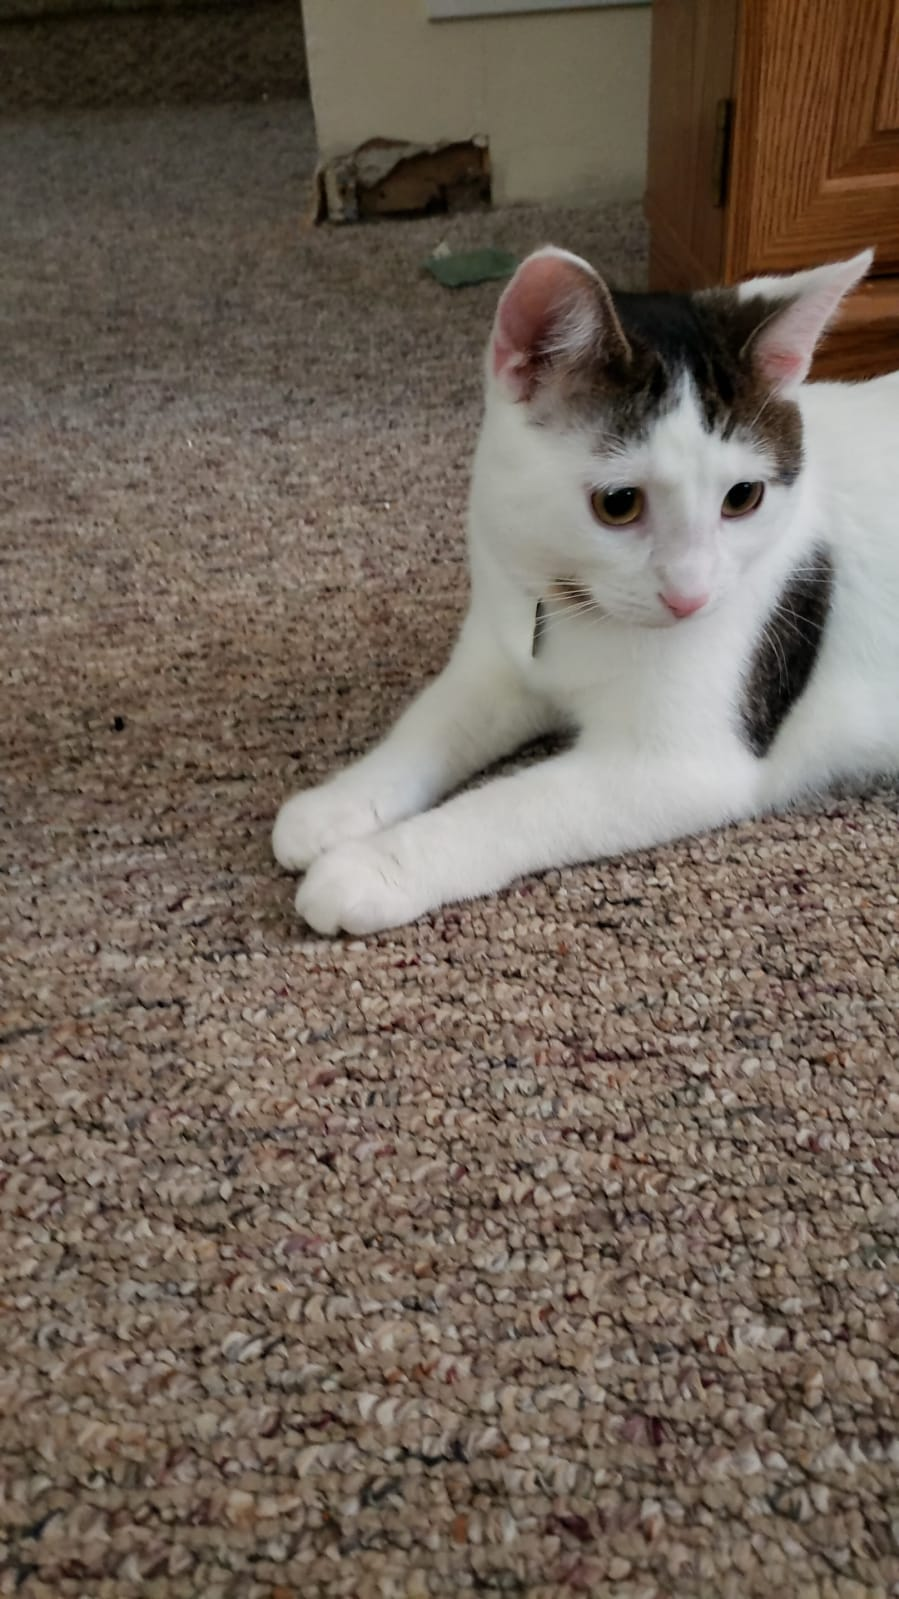
\includegraphics[scale=.2]{{./resources/cat2.jpg}}
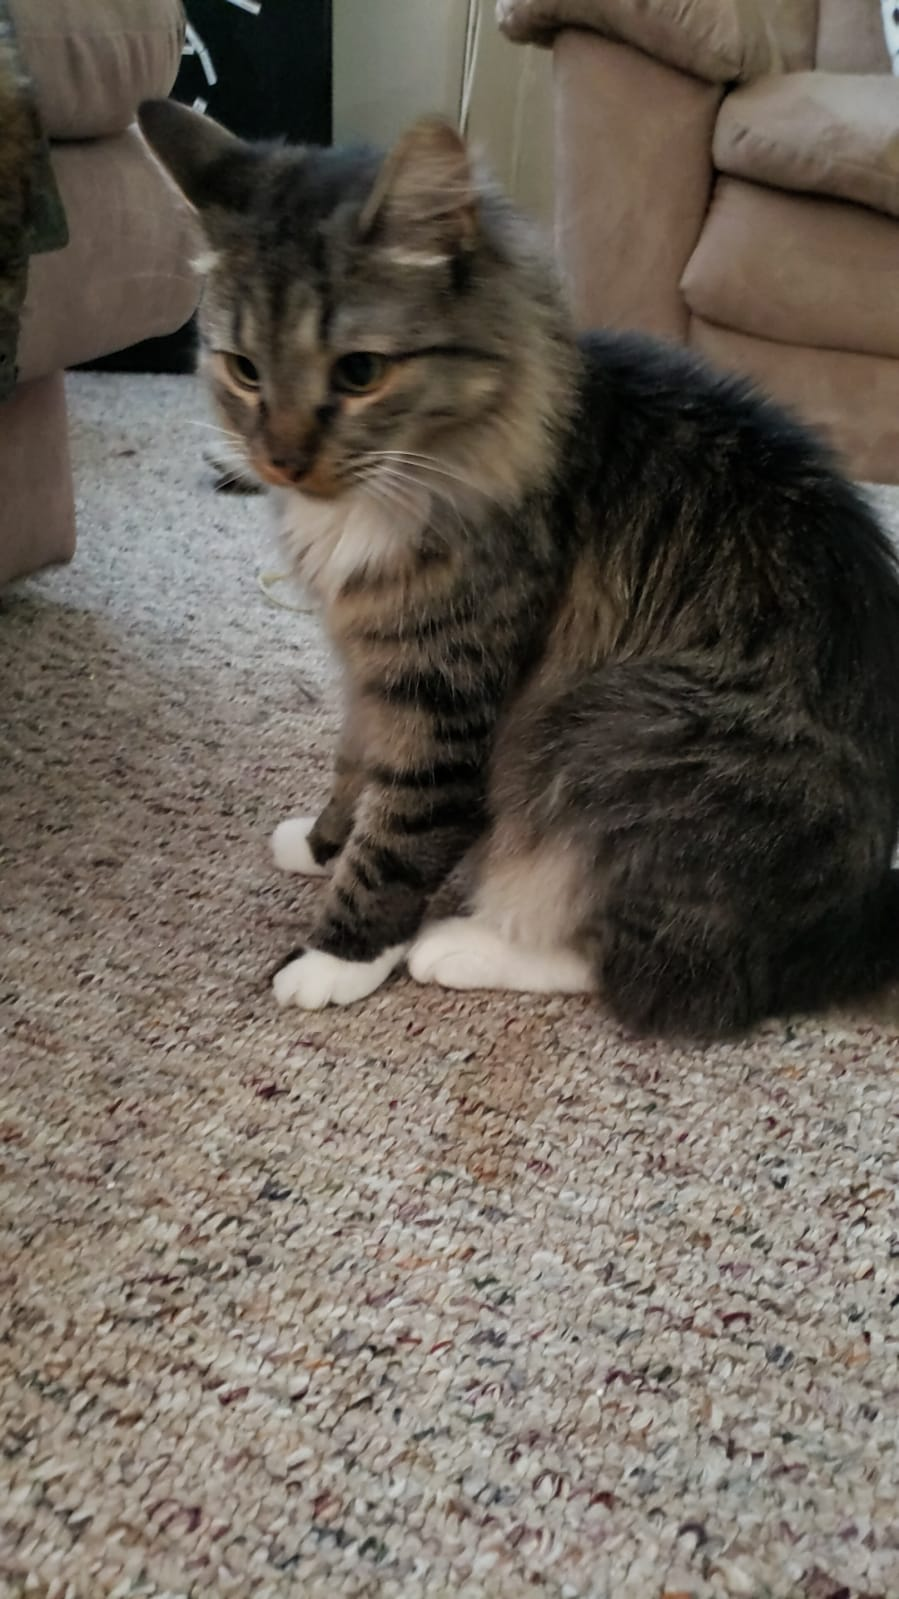
\includegraphics[scale=.2]{{./resources/cat1.jpg}} \\
Then we can continue words below... so seamless! On a side note, what do you think they're looking at :) Adding pictures in this way is good for other things aside from cats too, you can also add other important information as well!\\
\begin{minipage}{0.3\textwidth}
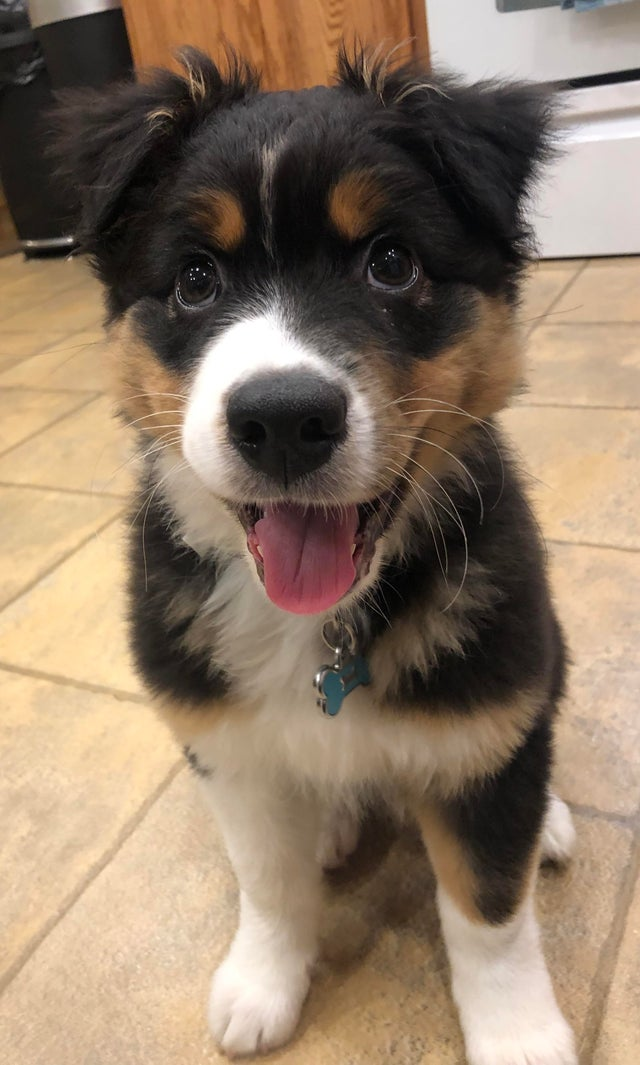
\includegraphics[width=\linewidth]{{./resources/puppy.jpg}}
\end{minipage}
\begin{minipage}{0.7\textwidth}
Not only can we have this adorable puppy, but the text can be aligned to the right of the picture so we can talk about everything in great detail while still maintaining an acceptable format! Ok well maybe this picture is a bad example because it's a bit too tall and I've run out of things to say about it so lets' try another instead.
\end{minipage}
\\
\begin{minipage}{0.7\textwidth}
Not 5 minutes ago I didn't even know you could do this with LaTeX... I'm literally entertaining myself on a Sunday night writing about nothing in a template document ... please send help haha Regardless this could come in handy when you've got multiple DOF pictures that might need to be displayed in the thesis and you want to get all fancy about it!
\end{minipage}
\begin{minipage}{0.3\textwidth}
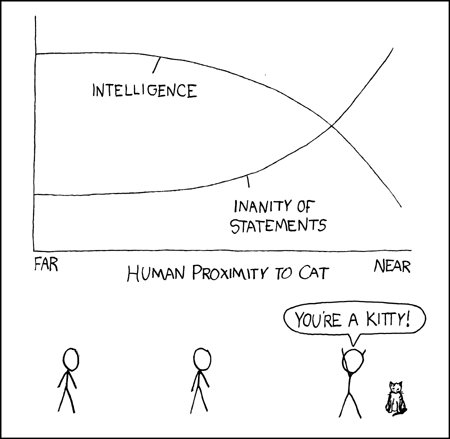
\includegraphics[width=\linewidth]{{./resources/cat_proximity.png}}
\end{minipage}

\subsection{How the Turn Tables}
I'll admit tables are a complete pain in the butt, but (hehe) there's an amazing website here: \chref{https://www.tablesgenerator.com/}{Something 
Linky} where you can input things are have it do custom formatting! If you do check the code to do even a simple table like this you'll know why I use that website lol

\begin{table}[htb]
\centering
\caption{Amazing Table with Purely Objective Data}
\begin{tabular}{|c|l|cccc|}
\hline
\textbf{Name}               & \multicolumn{1}{c|}{\textbf{Artist}} & \textbf{Beepiness} &  \textbf{Boopiness} & \textbf{Sad Factor} & \textbf{Rating}  \\ \hline
Flowers            & Ra Ra Riot                  & N/A       & 2/10      & 0/10       & 11/10   \\
Sky Full Of Stars  & Coldplay                    & 1/10      & 3/10      & 0/10       & 8/10    \\
Sleep on The Floor & Lumineers                   & 0/10      & 4/10      & :'(        & 10.5/10 \\
Sleepless Nights   & Nightly                     & 2/10      & 3/10      & 4/10       & $\lim\limits_{x \rightarrow 11} \frac{x}{10}$     \\ \hline
\end{tabular}
\end{table}



\section{Conclusion}
We've finally made it to the conclusion, I've pretty well covered all the major points I needed to cover and I already added a giant wall of random text in the intro so I'll keep this short! lol Hopefully you read that part all the way to the end too because I want to flex my baking muscle... who am I kidding I'm terrible at baking. I can cook amazing pad thai, seafood linguine, Chili, and many more things from scratch, but ask me to bake a pizza and it's all down hill from there. Oh and let me just clarify even pre-made oven pizzas I've been known to destroy haha Oh yes it's that bad! I did however attempt some GF bread once and aside from the fact that it came out about as dense as uranium it actually tasted outstanding... though I'll never do it again because that one loaf cost me almost \$ 25 to bake! But I digress if you've made it THIS far I'll even up the wager and attempt some artwork on my next card I send off. ;) You know what there is one other thing I forgot to address and this is the perfect setting, let's talk about that pastry! If the following description of the pastry isn't spot on for next week's adventure then I'll prepare an entire week's worth of lunches for you.
\paragraph{} Here we go, so it's a round pastry with a serrated, slightly raised edge which embodies the fan-blade arrangement of apple slices in the center. Upon first bite you're met with a slightly odd sensation that your mouth is about to become a desert, but amazingly it's not as dry as your senses first suggest. Though perhaps a bit crumbly it still manages to remain soft enough to not deter from the experience. Now if you've bitten far enough into the centre you'll notice that the pastry that's come into contact with the apple slices is actually a bit slimy, but not in a grotesque way as it's actually feigned the texture of the real thing! It's almost like there's a micro thin layer of apple jam holding everything together. In conclusion the pastry was an overall incredibly pleasant experience and I'd defintly return to the bakery to try their other treats!

\newpage
\bibliography{sources}
\bibliographystyle{ieeetr}

\end{document}